\chapter{Problemstellung}
In der heutigen Zeit, in der das weltweite Kommunikationsbedürfnis in ungeahnte Höhen steigt und, bis auf Weiteres, kein Ende des Anstiegs in Sicht ist, werden Computer-Netzwerke, besonders jene, welche ganze Kontinente umspannen, immer stärker beansprucht. Dieser Anstieg ist vor allem auf das gesteigerte und sich grundlegend ändernde Konsumverhalten der Menschen in der heutigen Zeit zurückzuführen. Immer mehr Informationen in Netzwerken werden nicht in Form von Texten sondern, aufwendig aufbereitet, als Bild und Ton zum Endkunden übertragen. Dieses Bild- und Tonmaterial erzeugt natürlich eine höhere Auslastung von Datenleitungen, was, im Zusammenspiel mit der gestiegenen Anzahl an Informationsbedürfnissen insgesamt, zu einer Verknappung der Ressourcen in Computer-Netzen führt.

Um diesen neuen Gegebenheiten gerecht zu werden gibt es zwei Möglichkeiten: entweder ein Ausbau und Neubau von Netzen, oder eine bessere Ausnutzung von bestehenden Netzen. Ausbau und Neubau bringen allerdings neue Probleme mit sich. Erstens ist Netzwerkinfrastruktur teuer, besonders wenn sie über mehrere Jahrzehnte hinweg halten und ihren Dienst verrichten soll ohne eine ständige Wartung mit sich zu ziehen. Zweitens ist es manchmal aus verschiedenen Gründen gar nicht möglich, ein Netz weiter auszubauen. Sollte sich eine bestehende Infrastruktur bereits in ihrer letzten Ausbaustufe befinden, ist es überhaupt notwendig ein gänzlich neues Netz aufzubauen, was wiederum mit noch höheren Kosten verbunden ist. Zu guter Letzt sorgt der Betrieb von zusätzlicher Infrastruktur auch für zusätzlichen Strombedarf, was sich nicht nur negativ auf die Kosten auswirkt, sondern durchaus auch eine Belastung für die Umwelt darstellt.

Die zweite Möglichkeit, die bessere Ausnutzung von bestehenden Netzen, kann zwar die letzt\-endliche Notwendigkeit von neuen Netzen nicht verhindern, den Zeitpunkt des Eintretens dieser letzten Option aber hinauszögern. Durch eine optimierte Nutzung können bereits vorhandene Netze über einen längeren Zeitraum genutzt werden ohne einen Engpass zu bilden. Wie diese Optimierungen im konkreten Fall aussehen hängt unter anderem von der Größe und der Art des Netzes, aber auch von der Art des Kommunikationsbedürfnisses ab. In dieser Arbeit konzentrieren wir uns auf rein optische Netze mit einer ganz genau definierten Art von Kommunikationsbedürfnissen.

In rein optischen Netzen, also Netzwerken, in denen Information als Lichtimpulse rein über optische Leiter wie Glasfaser übertragen wird und das Signal auf der ganzen Strecke zu keinem Zeitpunkt in ein elektrisches Signal zurück gewandelt wird, kann \textit{Wavelength Division Multiplexing} (WDM) zur parallelen Übertragung mehrerer Datenströme über ein und dieselbe Leitung betrieben werden. Die Idee hinter WDM ist es, für zwei verschiedene Datenströme unterschiedliche Farben des Lichts zu verwenden. Der englische Name Wavelength Division (deutsch: Wellenlängen Unterteilung) kommt von der Tatsache, dass verschiedene Farben des Lichts verschiedene, eindeutige Wellenlängen haben. Da sich die unterschiedliche Farben des Lichts bei entsprechendem Wellenlängenabstand nicht gegenseitig beeinflussen, können viele Farben gleichzeitig durch ein und denselben Lichtwellenleiter geschickt werden und am anderen Ende des Leiters wieder problemlos auseinander gehalten werden. Dies funktioniert sogar so gut, dass Lichtwellen, welche sich nur um wenige Nanometer an Wellenlänge unterscheiden, immer noch eindeutig zuordenbar sind.

Des Weiteren wird oft angestrebt, einem einzelnen Datenstrom auf seinem gesamten Weg durch das Netzwerk ein und dieselbe Farbe zu geben. Dies bietet Vorteil vor allem im Bereich der Einfachheit der Implementierung, da optische Switches innerhalb des Netzwerkes keine Umwandlung von einer Farbe in eine andere vornehmen müssen. Hinzu kommt ein geringerer Stromverbrauch im Netzwerk, da ein Umwandlung von einer Wellenlänge in eine andere auch ein gewisses Maß an zusätzlicher Energie benötigen würde.

Zu guter Letzt ist noch die spezielle Art des Kommunikationsbedürnisses zu beachten. Anders als zum Beispiel im Internet, wo die Kommunikation für einen Netzbetreiber unberechen- und vor allem unverhersehbar abläuft, gehen wir hier von einem Fall aus, in dem ein großter Teil der Kommunikationswünsche bereits von vornherein bekannt sind. Vorstellbar wäre solch ein Fall zum Beispiel bei einer gemieteten Standleitung eines Unternehmens zu dessen Zweigstelle am anderen Ende des Landes. Auch die Kommunikationsbedürfnisse zwischen Internetprovidern (z.\ B. Durchleitung von Daten) können im großen Maßstab als ein über einige Wochen oder Monate hinweg relativ konstantes Datenaufkommen betrachtet werden. Obwohl dies nun nach einer starken Einschränkung des Einsatzgebietes aussieht ist der Nutzen dennoch nicht zu unterschätzen. Wenn zum Beispiel der Aufwand für den Betrieb solcher Standleitungen minimiert werden kann, bleiben mehr Ressourcen des Netzwerkes frei für die Erfüllung der vorhin erwähnten unvorhersehbaren Kommunikationsbedürfnisse.

\section{Partition Graph Coloring Problem}
Mit Hilfe des \textit{Partition Graph Coloring Problems} (PCP) wird versucht, diesen sehr spezifischen Anwendungsfall mathematisch zu beschreiben. Um das Problem zu lösen wird ein Graph aufgebaut, mit dessen Hilfe dann eine möglichst gute, wenn nicht sogar optimale Lösung für das Problem berechnet werden kann. Ein Graph ist ein mathematisches Konstrukt, das aus Knoten besteht, die durch Kanten verbunden werden. Ein Knoten A kann mit Knoten B durch so eine Kante verbunden werden, Knoten A muss aber zum Beispiel keine Verbindung mit Knoten C besitzen. Wie schon von \citet*{Li2000} gezeigt wurde, handelt es sich bei dem PCP um ein NP-hartes Problem, das heißt es kann nicht in polynomieller Laufzeit auf einem Computer wie man ihn heute kennt eine Lösung gefunden werden, welche mit 100\%-iger Sicherheit die optimale Lösung für das konkrete Problem darstellt. Polynomielle Laufzeit wird im Normalfall als Grenze zwischen Problemen angesehen, welche in vertretbarer Laufzeit noch zu berechnen sind und Problemen, für die der Lösungsaufwand in keinem Verhältnis zum Ergebnis steht, namentlich, deren Laufzeit ein exponentielles Verhalten an den Tag legt.

\begin{figure}
	\centering
	\begin{subfigure}{\textwidth}
		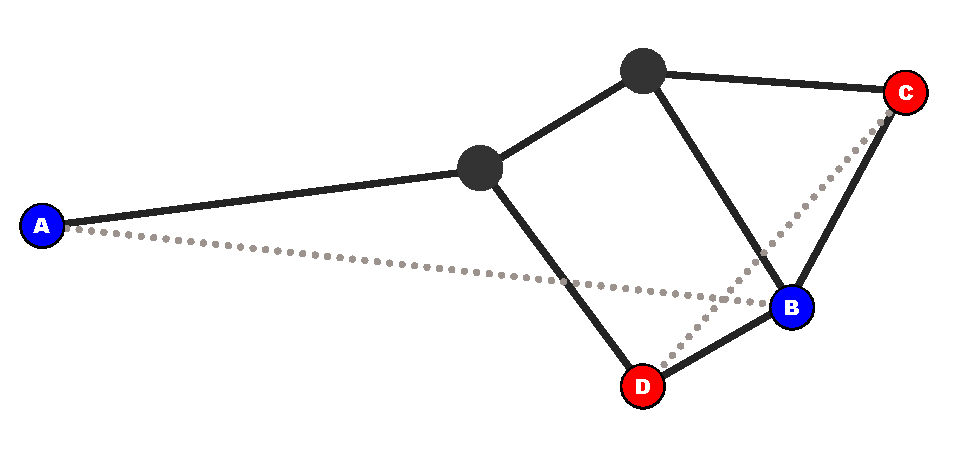
\includegraphics{img/bsp1}
		\caption{Repräsentatives Beispiel für ein rein optisches Netzwerk innerhalb Österreichs. Es gibt zwei Kommunikationswünsche und zwar zwischen A und B sowie zwischen C und D.}
		\label{fig:example:a}
	\end{subfigure}
	\begin{subfigure}{\textwidth}
		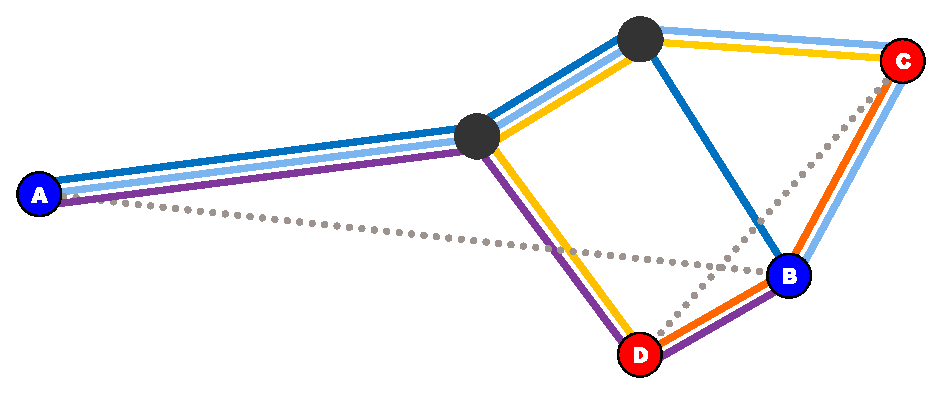
\includegraphics{img/bsp2}
		\caption{Beispiel für verschiedene Routen zwischen insgesamt vier Kommunikationspartnern. Verschiedene Möglichkeiten der Wegfindung zwischen A und B werden in Hell- und Dunkelblau sowie Violett dargestellt. Die alternativen Routen zwischen C und D sind gelb und orange eingefärbt.}
		\label{fig:example:b}
	\end{subfigure}
	\caption{Ein Beispiel für eine Probleminstanz des Partition Graph Coloring Problems}
	\label{fix:example}
\end{figure}

\begin{figure}
	\centering
	\begin{subfigure}[t]{0.3\textwidth}
		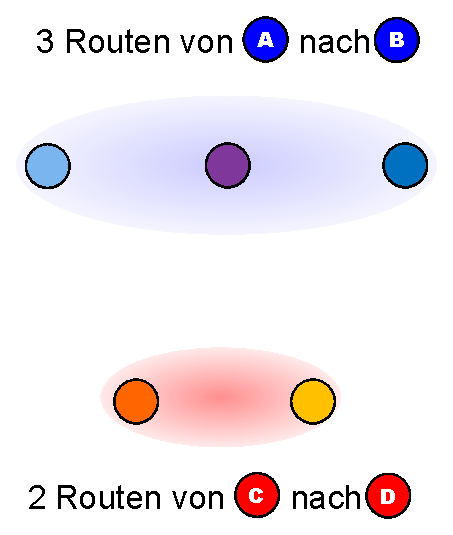
\includegraphics[width=\textwidth]{img/bsp3}
		\caption{Der aus Abbildung~\ref{fig:example:b} generierte Konfliktgraph. Jede Route wird als Knoten repräsentiert. Die verwendete Farbe stimmt mit den für die Routen verwendeten Farben überein. Die Partitionierung wird durch das Oval im Hintergrund der Knoten angedeutet.}
		\label{fig:example:c}
	\end{subfigure}
	\begin{subfigure}[t]{0.3\textwidth}
		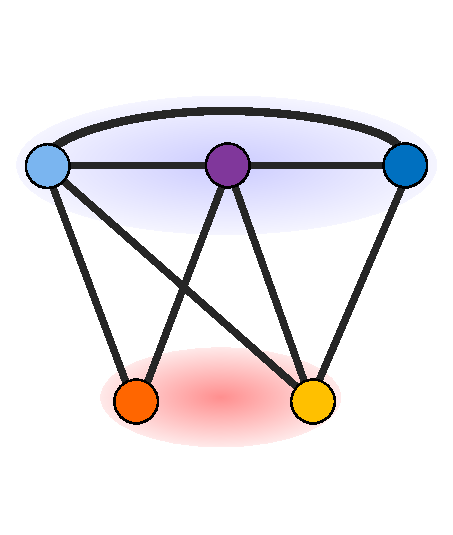
\includegraphics[width=\textwidth]{img/bsp4}
		\caption{Der Konfliktgraph wird um die Beziehungen der Knoten untereinander erweitert. Jede Route, welche eine Teilstrecke mit einer anderen Route gemeinsam hat, wird mit dieser Route verbunden. Die Kanten zwischen den Knoten stellen diese Beziehung dar.}
		\label{fig:example:d}
	\end{subfigure}
	\begin{subfigure}[t]{0.3\textwidth}
		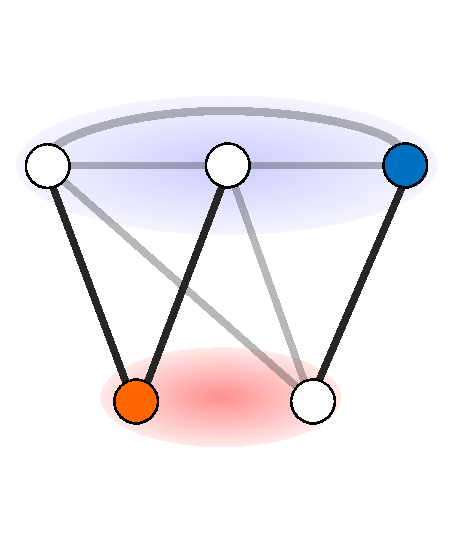
\includegraphics[width=\textwidth]{img/bsp5}
		\caption{Eine mögliche Lösung des PCP\@. Von jeder Partition muss nur ein Knoten ausgewählt werden, alle anderen werden ausgeblendet. Die Auswahl für die Strecke zwischen A und B hat kein gemeinsames Teilstück mit der für die Strecke C-D getroffenen Auswahl. Daher kann ein und dieselbe Wellenlänge für beide Übertragungen verwendet werden.}
		\label{fig:example:e}
	\end{subfigure}
	
	\caption{Aufbau und Lösung eines Problem-Graphen des Partition Graph Coloring Problems}
\end{figure}

Um das Problem besser lösen zu können, wird ein einheitliches Ziel und eine einheitliche Eingabe benötigt. Dazu wird die Problemstellung nun in einem ersten Schritt auf folgende Punkte fixiert:
\begin{itemize}
	\item Ein Netzwerk mit seinen möglichen Kommunikationsverbindungen zwischen den einzelnen Netzwerkknoten ist gegeben.
	\item Alle Kommunikationsbedürfnisse, welche aus einem Start- und einem Endpunkt bestehen, sind bekannt.
	\item Für jedes Kommunikationsbedürfnis gibt es einen oder mehrere Wege, sprich Routen, zwischen Start- und Endpunkt durch das Netzwerk.
	\item Sollte eine Route einen Teil des Weges auf der selben Strecke zurücklegen wie eine andere Route, müssen sie unterschiedliche Farben verwenden um sich nicht gegenseitig zu stören.
	\item Jede Route verwendet genau eine Farbe und zwar für die gesamte Strecke.
	\item Die Lösung besteht aus genau einer Route für jedes Kommunikationspaar und genau einer dazugehörigen Farbe.
\end{itemize}

Aus diesen Bedingungen kann ein Graph abgeleitet werden, der genau jene Bedürfnisse erfüllt, um ein einfaches Lösen des Problems zu ermöglichen. Der Konfliktgraph, auf dem dann die Lösung berechnet wird, besteht aus Partitionen, welche eine Menge von zusammengehörigen Knoten darstellt und Kanten, welche die einzelnen Knoten verbinden. Ein Kommunikationsbedürfnis zwischen zwei Partnern wird als eine Menge von Knoten gesehen. Die Knoten repräsentieren dabei je eine Route zwischen den beiden Partnern. Steht also nur eine Route zwischen zwei Kommunikationsendpunkten zur Auswahl, gibt es nur einen Knoten in dieser Menge. Diese Menge an Knoten wird Partition genannt und ist damit namensgebend für das PCP\@. Dieser Schritt wird in Abbildung~\ref{fig:example:c} veranschaulicht.

Die Kanten bilden nun die Beziehungen zwischen verschiedenen Routen ab. Teilen sich zwei Routen das selbe Teilstück im optischen Netzwerk, werden sie mit einer Kante verbunden. Zu beachten ist, dass dies nicht nur für Knoten in der selben Partition gilt sondern auch für Knoten aus unterschiedlichen Partitionen. Verwendet also Route $X$ der Kommunikation $(AB)$ ein Stück der Strecke, das auch von der Route $Y$ der Kommunikation $(CD)$ verwendet wird, werden diese beiden Routen, welche ja jeweils als Knoten repräsentiert werden, im Konfliktgraphen mit Hilfe einer Kante verbunden. Außerdem ist noch zu beachten, dass für jedes in dieser Art verbundene Routenpaar nur eine Kante verwendet wird. Teilen sich Routen $X$ und $Y$ mehr als ein Teilstück, so werden sie trotzdem nur einmal per Kante verbunden. Die Vervollständigung des Konfliktgraphen wird in Abbildung~\ref{fig:example:d} dargestellt.

Nachdem der Konfliktgraph generiert wurde, kann eine Lösung für das PCP berechnet werden. Für das durch die Partition symbolisierte Kommunikationsbedürfnis muss genau eine Route ausgewählt werden und diese Knoten müssen dann so eingefärbt werden, dass sich keine zwei mit einer Kante verbunden Knoten die gleiche Farbe teilen. Der letztere Teil, also das Einfärben von Knoten in Abhängigkeit der Farben der Nachbarknoten, ist als klassisches \textit{Graph Coloring} (GC) bekannt. Es kommt zum Beispiel bei der Einfärbung von politischen Landkarten zum Einsatz, wo benachbarte Länder nicht die selbe Farbe haben dürfen. Was das PCP vom klassichen GC unterscheidet, ist die zusätzliche Aufgabe, nur einen Knoten aus einer Partition als Repräsentanten auszuwählen und die anderen quasi auszublenden. Ein Beispiel einer solchen Lösung des Problems ist in Abbildung~\ref{fig:example:e} zu finden.

Die Schwierigkeit des Problems liegt in dem Zusammenspiel von verschiedenen Möglichkeiten, ein und den selben Graphen einzufärben und andererseits mit einer anderen Auswahl an Knoten gleich den gesamten Lösungsgraphen zu verändern. Das Kriterium für die Güte einer Lösung ist die Anzahl der verwendeten Farben. Im Originalproblem entspricht das der Anzahl an Wellenlängen, die für die vorab bekannte Kommunikation im Netzwerk benötigt werden. Um sich nur auf diese Anzahl konzentrieren zu können, wird angenommen, dass jede Route zwischen zwei Kommunikationspartnern gleich gut ist. Eventuelle Umwege (Routen länger als die kürzeste mögliche) werden also im PCP ignoriert. 

Außerdem geht man bei der Lösung des PCP von einem homogenen Netzwerk aus, in dem jede Leitung jede Wellenlänge unterstützt. In der Realität kann es durchaus vorkommen, dass ein Lichtwellenleiter, welcher aus einem chemisch minimal anders zusammengesetzten Stoff besteht als seine Gegenstücke in anderen Teilen des Netzwerkes, für bestimmte Wellenlängen ungünstige Eigenschaften hat. Dieser Aspekt wird beim Lösen des PCP nicht beachtet, jede Strecke beziehungsweise jede Route unterstützt alle Wellenlängen. Außerdem wird angenommen, dass jeder Leiter eine unbegrenzte Anzahl an Wellenlängen unterstützt. Reale Leiter können nur eine begrenzte Anzahl an Wellenlängen unterstützen, bis ihr Spektrum ausgeschöpft ist.

\subsection{Formale Definition}

Gegeben sei ein ungerichteter Graph $G = (V,\ E)$, wobei $V$ die Menge der Knoten des Graphen $G$ und $E$ die Men\-ge der Kan\-ten, die $V$ in $G$ verbinden, darstellen. Außerdem seien $V_1,\ V_2,\ V_3,\ \ldots,$ $V_k$ disjunkte Teilmengen von $V$ $V_i \cap V_j = \emptyset \ \forall i,\ j = 1,\ \ldots,\ k$ mit $i \not = j$, wobei $\bigcup_{i = 1}^k V_i = V$ welche folgend \textit{Partition} oder auch \textit{Komponente} genannt werden.

Das \textit{Partition Graph Coloring Problem} (PCP) besteht nun darin, eine Menge $V'$ zu finden, sodass $|V' \cap V_i| = 1,\ \forall\ i = 1,\ \ldots,\ k$ gilt ($V'$ also genau einen Knoten für jede Partition enthält) und weiter die Färbung $S$ des durch die Menge $V'$ und der für $E$ implizierten Untermenge an Kanten $E'$ konstruierbaren Graphen $G' = (V', E')$ minimal ist.

Als Lösung des Problems kann die Menge der \textit{Repräsentanten} in $V'$ gemeinsam mit deren Färbung $S$ angesehen werden.

\section{Ausgangsmaterial}
Das Partition Graph Coloring Problem beschränkt sich nur auf den Weg vom Konfliktgraphen zum Lösungsgraphen. Für die Findung alternativer Routen durch ein Netzwerk gibt es 
bereits ausgiebig beschriebene und getestete Algorithmen, welche auch auf ein optisches Netzwerk anwendbar sind. Mit Hilfe dieser Algorithmen (z.\ B. kürzeste Wege Algorithmen) können die für den
Konfliktgraphen benötigten Knoten für jedes Kommunikationspaar gefunden werden. Wichtig hierbei ist es, dass es wenn möglich mehrere Alternativen für eine Übertragung geben sollte,
da es sich sonst um ein normales Graph Coloring Problem handeln würde. Die Findung der Kanten, welche Knoten verbinden, die die selbe Teilstrecke verwenden, ist auch ein
gelöstes Problem, welches das PCP nicht beschäftigt.

Das PCP generiert eine Lösung aus dem Konfliktgraphen, welche eindeutig für jeden Kommunikationswunsch eine Route wählt und dieser eine Farbe zuordnet. Je dichter der Konfliktgraph, das heißt
je mehr Kanten die verschiedenen Knoten verbinden, desto schwieriger ist es, eine geringe Anzahl an Farben für die optimierte Lösung zu finden. Dabei legt ein Algorithmus, der das
PCP löst, nicht strikt die zu verwendenden Wellenlängen fest, sondern weist gleichen Wellenlängen nur die gleiche Zahl zu. Gleiches gilt für die Auswahl einer Route. Anstelle
einer fixen Beschreibung, welchen Weg die ausgewählte Route durch das Netzwerk nimmt, zeigt ein Algorithmus für das PCP lediglich auf, welcher Knoten verwendet wurde. 
Die Zuordnung von Knoten zur Route muss daher, wie auch schon bei den Wellenlängen, später erfolgen.

\section{Bisherige Ansätze}
Bevor die in dieser Arbeit verwendete Lösungsstrategie für das PCP erläutert wird soll kurz erwähnt werden welche Lösungsansätze zu Beginn der Diplomarbeit evaluiert wurden.

\subsection{Heuristisch}
\label{sec:li2000}
\citet*{Li2000} definieren das PCP, beweisen, dass das Problem NP-schwierig ist und vergleichen verschiedene heuristische Ansätze. Aufgrund der Ergebnisse des Vergleichs wurde die Konstruktionsheuristik für die Variable Nachbarschaftssuche gewählt (sie\-he Abschnitt~\ref{sec:construct}).

\subsection{Metaheuristisch}
\label{sec:tabu}
\citet*{Noronha2006} beschreiben eine Tabu-Suche, ein iteratives metaheuristisches Verfahren, welche durchnschnittlich um 20\% bessere Ergebnisse liefern als die in Abschnitt~\ref{sec:li2000} erwähnten Heuristiken.

\subsection{Exakt}
\citet*{Frota2010} zeigen einen Lösungsweg mithilfe von Branch-and-Cut und \citet*{Hoshino2011} einen mit Branch-and-Price. Beide basieren auf der \textit{ganzzahligen linearen Optimierung} (engl.\ \textit{integer linear programming}, ILP) und verfolgen einen fundamental anderen Lösungsansatz als erwähnte (Meta-)Heuristiken bzw.\ die in dieser Arbeit vorgestellten Variablen Nachbarschaftssuche.
